\chapter{The Universal Regime Map}
\label{ch:regime_map}

Every physical domain in the AVE framework reduces to a single dimensionless control parameter $r = A/A_c$, where $A$ is the local strain amplitude and $A_c$ is the domain-specific critical threshold derived from the four axioms. The saturation operator $S(r) = \sqrt{1 - r^2}$ (Axiom~4) changes character at well-defined boundaries, partitioning all of physics into four universal regimes.

This chapter establishes the regime classification as a \textbf{prerequisite gate}: no domain analysis proceeds without first identifying its regime and verifying the appropriate equation set.

\section{The Four Universal Regimes}

\begin{resultbox}{Universal Regime Classification}
\begin{equation}
    S(r) = \sqrt{1 - r^2}, \qquad r \equiv \frac{A}{A_c}
\end{equation}
\end{resultbox}

\begin{center}
\begin{tabular}{|c|l|c|c|l|}
\hline
\textbf{Regime} & \textbf{Name} & \textbf{$r$ range} & \textbf{$S$ range} & \textbf{Physics} \\ \hline
I   & Linear     & $r < 0.1$        & $S > 0.995$       & Standard equations (Maxwell, Newton) \\
II  & Nonlinear  & $0.1 \leq r < 0.9$ & $0.436 < S < 0.995$ & Axiom~4 corrections non-negligible \\
III & Yield      & $0.9 \leq r < 1.0$ & $0 < S < 0.436$   & Phase transition zone \\
IV  & Ruptured   & $r \geq 1.0$       & $S = 0$           & Topology destroyed \\ \hline
\end{tabular}
\end{center}

\noindent The boundary values (0.1, 0.9, 1.0) are not arbitrary:

\begin{itemize}
    \item \textbf{$r = 0.1$:} The perturbative expansion $S \approx 1 - r^2/2$ is accurate to $< 0.5\%$. Below this threshold, Axiom~4 corrections are negligible and all standard (Maxwell/Newton) results are recovered. No simulation needs the full nonlinear operator.

    \item \textbf{$r = 0.9$:} Below this threshold, $S$ varies smoothly. Above it, $S$ drops precipitously ($dS/dr \to -\infty$ as $r \to 1$), signaling a phase transition where the metric stiffens catastrophically. The quality factor $Q = 1/\sqrt{1-r^2}$ exceeds $2.3\times$ at $r = 0.9$, indicating measurable energy trapping.

    \item \textbf{$r = 1.0$:} The topology is destroyed. The saturation factor reaches zero, compliance vanishes, and the node can no longer support propagating waves. In different domains this manifests as: pair production (EM), event horizon formation (gravity), quark deconfinement (nuclear), or superconducting transition (BCS).
\end{itemize}

\subsection{Perturbative Expansion (Regime~I)}

In Regime~I, the saturation factor admits a convergent Taylor expansion:
\begin{equation}
    S(r) = 1 - \frac{r^2}{2} - \frac{r^4}{8} - \frac{r^6}{16} - \cdots
    \label{eq:S_taylor}
\end{equation}
To leading order, $\Delta S \approx r^2/2$. For $r = 0.1$, $\Delta S < 0.005$ ($0.5\%$). This validates the use of unmodified Maxwell/Newton equations in all terrestrial laboratory experiments except those explicitly designed to approach $V_{yield}$ (e.g., PONDER-05).

\section{Domain Control Parameter Catalog}
\label{sec:domain_catalog}

Each domain has a unique physical interpretation of the amplitude $A$ and the critical threshold $A_c$. In every case, $A_c$ is \textbf{derived from the four axioms}---it is never a fitted or empirical parameter.

\subsection{Electromagnetic (Dielectric)}

\begin{center}
\begin{tabular}{ll}
\toprule
Amplitude $A$ & Applied voltage $V$ \\
Critical $A_c$ & $V_{yield} = \sqrt{\alpha} \cdot V_{snap} = \sqrt{\alpha} \cdot m_e c^2/e \approx 43.65$ kV \\
Control parameter & $r = V / V_{yield}$ \\
\bottomrule
\end{tabular}
\end{center}

\noindent \textbf{Regime locations:}
\begin{itemize}
    \item Lab capacitor (1~kV): $r = 0.023$ --- Regime~I
    \item PONDER-05 @ 30~kV: $r = 0.687$ --- Regime~II
    \item PONDER-05 @ 43~kV: $r = 0.985$ --- Regime~III
    \item Schwinger pair production: $r = 1.0$ --- Regime~IV boundary
\end{itemize}

\subsection{Electromagnetic (Field Strength)}

\begin{center}
\begin{tabular}{ll}
\toprule
Amplitude $A$ & Local electric field $E$ \\
Critical $A_c$ & $E_{yield} = V_{yield}/\ell_{node} \approx 1.13 \times 10^{17}$ V/m \\
Control parameter & $r = E / E_{yield}$ \\
\bottomrule
\end{tabular}
\end{center}

\noindent At the lattice scale, even extreme laboratory fields ($10^6$~V/m) correspond to $r \sim 10^{-11}$, deep in Regime~I. The Schwinger critical field ($E_S = m_e^2 c^3/(e\hbar) \approx 1.32 \times 10^{18}$~V/m) corresponds to $r = E_S/E_{yield} = V_{snap}/V_{yield} = 1/\sqrt{\alpha} \approx 11.7$, deep in Regime~IV.

\subsection{Gravitational}

\begin{center}
\begin{tabular}{ll}
\toprule
Amplitude $A$ & Principal radial strain $\varepsilon_{11} = 7GM/(c^2 r)$ \\
Critical $A_c$ & Unitary strain = 1 \\
Control parameter & $r = \varepsilon_{11}$ \\
\bottomrule
\end{tabular}
\end{center}

\noindent The factor of 7 arises from the 7 compliance modes of the K4/SRS lattice ($\nu_{vac} = 2/7$). \textbf{Regime locations:}
\begin{itemize}
    \item Solar surface: $\varepsilon_{11} = 2.1 \times 10^{-6}$ --- Regime~I
    \item White dwarf: $\varepsilon_{11} \approx 3 \times 10^{-4}$ --- Regime~I
    \item Neutron star (1.4~$M_\odot$, $R = 10$~km): $\varepsilon_{11} \approx 1.46$ --- Regime~IV
    \item Black hole at $r_s = 2GM/c^2$: $\varepsilon_{11} = 7/2 = 3.5$ --- Regime~IV
\end{itemize}

\noindent \textit{The neutron star result demands attention.} A 1.4~$M_\odot$ star at $R = 10$~km has $\varepsilon_{11} = 1.46 > 1$, placing it in Regime~IV (ruptured topology). This is the AVE analog of the Buchdahl limit: no static configuration can have $r < 9GM/4c^2$ (where $\varepsilon_{11} > 63/36 = 1.75$). In AVE, the saturation boundary defines an absolute limit on gravitational compactness --- the lattice topology cannot support strain beyond unity.

\subsection{BCS / Superconducting}

\begin{center}
\begin{tabular}{ll}
\toprule
Amplitude $A$ & Temperature $T$ (or magnetic field $B$) \\
Critical $A_c$ & $T_c$ (or $B_{c0}$) \\
Control parameter & $r = T/T_c$ \\
\bottomrule
\end{tabular}
\end{center}

\noindent The BCS relation $B_c(T) = B_{c0}\sqrt{1 - (T/T_c)^2}$ IS the AVE saturation operator, with $A = T$ and $A_c = T_c$. Below $T_c$: superconducting ($S > 0$, Meissner effect active). At $T_c$: normal state ($S = 0$, topology destroyed).

\subsection{Magnetic}

\begin{center}
\begin{tabular}{ll}
\toprule
Amplitude $A$ & Applied magnetic field $B$ \\
Critical $A_c$ & $B_{snap} = m_e^2 c^2/(e\hbar) \approx 1.89 \times 10^9$ T \\
Control parameter & $r = B / B_{snap}$ \\
\bottomrule
\end{tabular}
\end{center}

\noindent Lab magnets ($\sim$10~T) have $r \sim 10^{-8}$ (Regime~I). A magnetar surface field ($\sim 10^{10}$~T) has $r \sim 5$ (Regime~IV). At $B_{snap}$, the vacuum permeability $\mu_{eff}$ reaches zero --- the vacuum becomes a perfect diamagnet (the Meissner effect of the vacuum itself).

\subsection{Nuclear}

\begin{center}
\begin{tabular}{ll}
\toprule
Amplitude $A$ & $d_{sat}/r_{sep}$ (confinement ratio) \\
Critical $A_c$ & 1 (Pauli wall) \\
Control parameter & $r = d_{sat}/r_{sep}$ \\
\bottomrule
\end{tabular}
\end{center}

\noindent When $r_{sep} > d_{sat}$: $r < 1$, the interaction potential $U(r) = -(K/r)(1 - 2\Gamma^2)$ is attractive (Regime~I--III). When $r_{sep} \leq d_{sat}$: $r \geq 1$, $\Gamma \to 1$, the potential becomes repulsive --- this is Pauli exclusion from first principles.

\subsection{Gravitational Waves}

\begin{center}
\begin{tabular}{ll}
\toprule
Amplitude $A$ & GW strain $h$ \\
Critical $A_c$ & $h_{yield} = \sqrt{\alpha} \approx 0.0854$ \\
Control parameter & $r = h / \sqrt{\alpha}$ \\
\bottomrule
\end{tabular}
\end{center}

\noindent LIGO detections ($h \sim 10^{-21}$) correspond to $r \sim 10^{-20}$ --- the most deeply linear measurement in physics. A neutron star merger at the surface ($h \sim 0.01$) reaches $r \sim 0.12$ (Regime~II).

\subsection{Galactic Rotation}

\begin{center}
\begin{tabular}{ll}
\toprule
Amplitude $A$ & Newtonian gravitational acceleration $g_N$ \\
Critical $A_c$ & $a_0 \approx 1.2 \times 10^{-10}$ m/s$^2$ \\
Control parameter & $r = g_N / a_0$ \\
\bottomrule
\end{tabular}
\end{center}

\noindent \textit{Note:} The galactic domain has an \textbf{inverted} interpretation. High $g_N$ (inner galaxy) means $r \gg 1$ --- deep Regime~IV, where the saturation correction is negligible (the Newtonian potential dominates). Low $g_N$ (outer galaxy) means $r \to 0$ --- but this is the deep MOND limit where the lattice compliance gradient produces the $\sqrt{g_N a_0}$ effective acceleration. The rotation curve flattening occurs at $r \sim 1$ (Regime~III).

\section{Regime-Specific Equation Sets}

For each regime, the constitutive parameters simplify:

\begin{center}
\begin{tabular}{|l|c|c|c|c|}
\hline
\textbf{Quantity} & \textbf{I (Linear)} & \textbf{II (Nonlinear)} & \textbf{III (Yield)} & \textbf{IV (Ruptured)} \\ \hline
$\varepsilon_{eff}$ & $\varepsilon_0$ & $\varepsilon_0 \sqrt{1-r^2}$ & $\to 0$ & 0 \\
$\mu_{eff}$         & $\mu_0$         & $\mu_0 \sqrt{1-r^2}$         & $\to 0$ & 0 \\
$c_{eff}$           & $c_0$           & $c_0(1-r^2)^{1/4}$          & $\to 0$ & 0 \\
$Z_{eff}$           & $Z_0$           & $Z_0 / (1-r^2)^{1/4}$       & $\to \infty$ & $\infty$ \\
$C_{eff}$           & $C_0$           & $C_0 / \sqrt{1-r^2}$        & $\to \infty$ & $\infty$ \\
$Q$                 & $\sim 1$        & $1/\sqrt{1-r^2}$             & $\gg 1$      & $\infty$ \\ \hline
\end{tabular}
\end{center}

\noindent The symmetric saturation case (both $\varepsilon$ and $\mu$ collapse equally) preserves $Z = \sqrt{\mu/\varepsilon} = Z_0$ (impedance invariant), while the asymmetric case (one collapses before the other) drives $Z$ to either 0 or $\infty$. The symmetric case governs gravity; the asymmetric case governs particle confinement (Meissner-like $\mu \to 0$ first $\Rightarrow Z \to 0$, $\Gamma \to -1$, standing wave $=$ rest mass).

\section{Cross-Domain Dimensional Analysis}
\label{sec:dimensional_analysis}

In every domain, when expressed in terms of the dimensionless control parameter $r$, the equations of motion take the same form:
\begin{resultbox}{Universal Dimensionless Master Equation}
\begin{equation}
    \frac{\partial^2 \phi}{\partial t^2} = c_0^2 (1-r^2)^{1/2} \nabla^2 \phi
\end{equation}
\end{resultbox}
where $\phi$ is the generalized displacement field (voltage, strain, temperature, GW perturbation) and $r = A/A_c$ is the domain-specific control parameter. This is a single equation governing all of physics; the domain merely specifies the physical meaning of $\phi$, $A$, and $A_c$.

\section{The Experimental Design Space}

Figure~\ref{fig:regime_design_space} maps every AVE experiment and astrophysical benchmark onto the regime diagram.

\begin{center}
\begin{tabular}{|l|c|c|c|}
\hline
\textbf{Object / Experiment} & \textbf{Domain} & \textbf{$r$} & \textbf{Regime} \\ \hline
\multicolumn{4}{|c|}{\textit{Regime I (Linear, $r < 0.1$)}} \\ \hline
LIGO GW150914              & GW       & $10^{-20}$ & I \\
Solar surface              & Gravity  & $2 \times 10^{-6}$  & I \\
Lab capacitor (1~kV)       & EM       & $0.023$    & I \\
MRI scanner (3~T)          & Magnetic & $10^{-9}$  & I \\
\hline
\multicolumn{4}{|c|}{\textit{Regime II (Nonlinear, $0.1 \leq r < 0.9$)}} \\ \hline
PONDER-05 @ 30~kV          & EM       & $0.687$    & II \\
Nb superconductor @ 4~K    & BCS      & $0.435$    & II \\
NS merger surface ($h \sim 0.01$) & GW & $0.117$    & II \\
\hline
\multicolumn{4}{|c|}{\textit{Regime III (Yield, $0.9 \leq r < 1.0$)}} \\ \hline
PONDER-05 @ 43~kV          & EM       & $0.985$    & III \\
Nb @ 9.1~K ($T_c = 9.2$~K) & BCS    & $0.989$    & III \\
\hline
\multicolumn{4}{|c|}{\textit{Regime IV (Ruptured, $r \geq 1.0$)}} \\ \hline
Neutron star ($1.4 M_\odot$, 10~km) & Gravity & $1.46$ & IV \\
Black hole at $r_s$        & Gravity  & $3.50$     & IV \\
Magnetar ($10^{10}$~T)     & Magnetic & $5.29$     & IV \\
Schwinger field             & EM      & $11.7$     & IV \\
\hline
\end{tabular}
\end{center}

\begin{figure}[H]
    \centering
    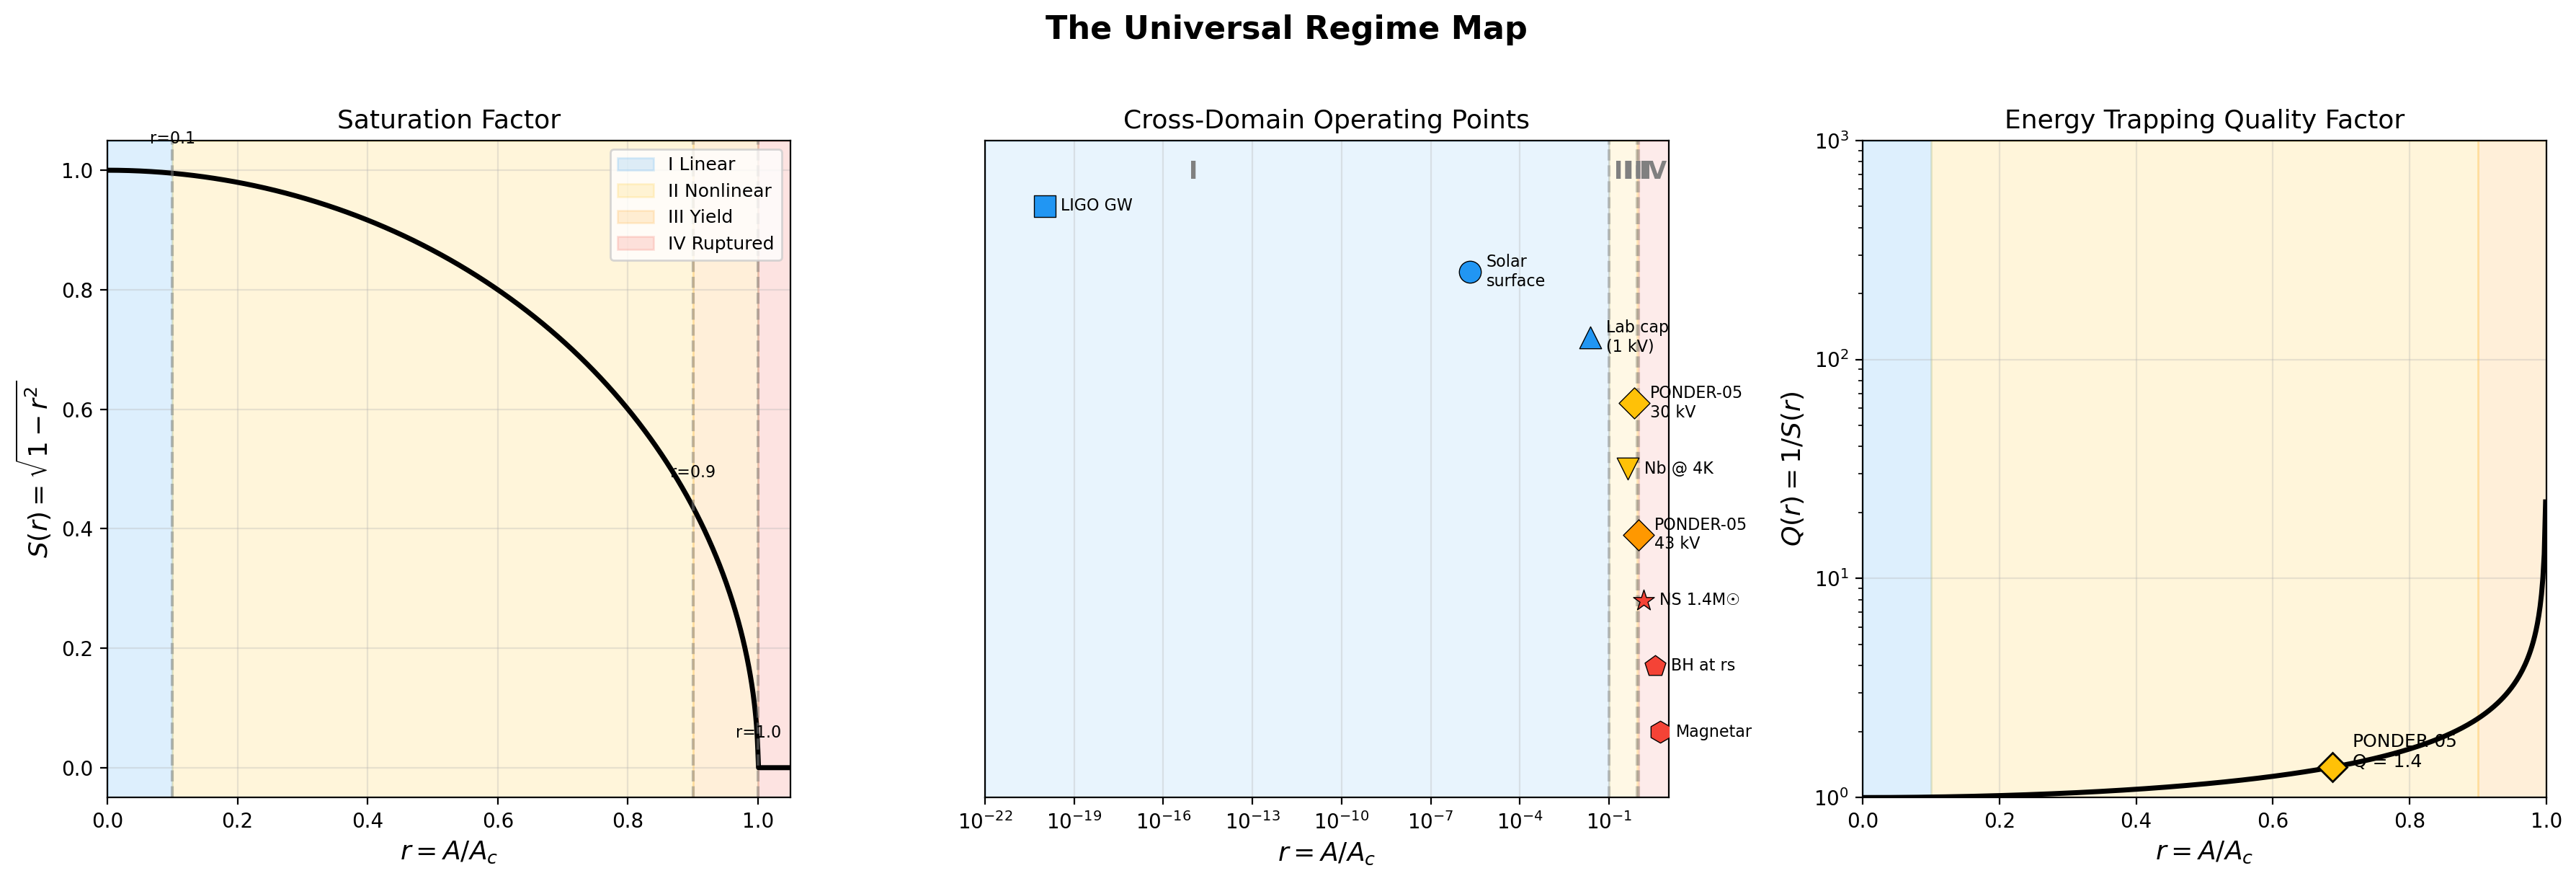
\includegraphics[width=1.0\textwidth]{regime_map.png}
    \caption{\textbf{The Universal Regime Map.} The saturation factor $S(r)$ (left axis) and energy trapping quality factor $Q = 1/S$ (right axis) as functions of the dimensionless control parameter $r = A/A_c$. The four regimes are shaded: blue (Linear), yellow (Nonlinear), orange (Yield), red (Ruptured). Physical operating points from all eight domains are marked. Every experiment and astrophysical object in the AVE framework is locatable on this single diagram.}
    \label{fig:regime_design_space}
\end{figure}
